\documentclass[11pt]{article}

\usepackage[T1]{fontenc}
\usepackage[utf8]{inputenc}
\usepackage{lmodern}
\usepackage[margin=1in]{geometry}
\usepackage{amsmath,amssymb}
\usepackage{booktabs}
\usepackage{graphicx}
\usepackage{multirow}
\usepackage{xcolor}
\usepackage[numbers,sort&compress]{natbib}
\usepackage[colorlinks=true,linkcolor=black,citecolor=blue!50!black,urlcolor=blue!50!black]{hyperref}
\usepackage{caption}
\captionsetup{font=small,labelfont=bf}
\emergencystretch=1.5em

\newcommand{\rattBcLateC}{57.5}
\newcommand{\rattBcLateCL}{59.1}
\newcommand{\rattBcLateLXXX}{56.5}
\newcommand{\rattBcLongC}{57.2}
\newcommand{\rattBcLongCL}{59.0}
\newcommand{\rattBcLongLXXX}{56.3}
\newcommand{\rattBcShortC}{56.3}
\newcommand{\rattBcShortCL}{58.7}
\newcommand{\rattBcShortLXXX}{55.0}
\newcommand{\rattCtlLateC}{57.2}
\newcommand{\rattCtlLateCL}{59.1}
\newcommand{\rattCtlLateLXXX}{56.6}
\newcommand{\rattCtlLongC}{57.2}
\newcommand{\rattCtlLongCL}{59.1}
\newcommand{\rattCtlLongLXXX}{56.3}
\newcommand{\rattCtlShortC}{56.4}
\newcommand{\rattCtlShortCL}{58.7}
\newcommand{\rattCtlShortLXXX}{54.8}
\newcommand{\rattEarlyBcC}{56.3}
\newcommand{\rattEarlyBcCL}{58.7}
\newcommand{\rattEarlyBcLXXX}{55.0}
\newcommand{\rattEarlyCtlC}{56.4}
\newcommand{\rattEarlyCtlCL}{58.7}
\newcommand{\rattEarlyCtlLXXX}{54.8}
\newcommand{\rattLateBcC}{57.5}
\newcommand{\rattLateBcCL}{59.1}
\newcommand{\rattLateBcLXXX}{56.5}
\newcommand{\rattLateCtlC}{57.2}
\newcommand{\rattLateCtlCL}{59.1}
\newcommand{\rattLateCtlLXXX}{56.6}
\newcommand{\rbluffBcLateC}{0.210}
\newcommand{\rbluffBcLateCL}{0.302}
\newcommand{\rbluffBcLateLXXX}{0.145}
\newcommand{\rbluffBcShortC}{0.212}
\newcommand{\rbluffBcShortCL}{0.301}
\newcommand{\rbluffBcShortLXXX}{0.151}
\newcommand{\rbluffCtlLateC}{0.211}
\newcommand{\rbluffCtlLateCL}{0.301}
\newcommand{\rbluffCtlLateLXXX}{0.142}
\newcommand{\rbluffCtlShortC}{0.211}
\newcommand{\rbluffCtlShortCL}{0.307}
\newcommand{\rbluffCtlShortLXXX}{0.150}
\newcommand{\rcorrBcLateC}{+0.029}
\newcommand{\rcorrBcLateCL}{+0.044}
\newcommand{\rcorrBcLateLXXX}{+0.009}
\newcommand{\rcorrBcShortC}{+0.059}
\newcommand{\rcorrBcShortCL}{\ensuremath{-}0.002}
\newcommand{\rcorrBcShortLXXX}{+0.020}
\newcommand{\rcorrCtlLateC}{\ensuremath{-}0.013}
\newcommand{\rcorrCtlLateCL}{+0.004}
\newcommand{\rcorrCtlLateLXXX}{+0.028}
\newcommand{\rcorrCtlShortC}{+0.025}
\newcommand{\rcorrCtlShortCL}{\ensuremath{-}0.003}
\newcommand{\rcorrCtlShortLXXX}{+0.045}
\newcommand{\rcorrPLateC}{0.099}
\newcommand{\rcorrPLateCL}{0.189}
\newcommand{\rcorrPLateLXXX}{0.509}
\newcommand{\rcorrPShortC}{0.426}
\newcommand{\rcorrPShortCL}{0.983}
\newcommand{\rcorrPShortLXXX}{0.494}
\newcommand{\rcorrWindow}{50}
\newcommand{\rcovertBcLateC}{0.291}
\newcommand{\rcovertBcLateCL}{0.199}
\newcommand{\rcovertBcLateLXXX}{0.353}
\newcommand{\rcovertBcShortC}{0.279}
\newcommand{\rcovertBcShortCL}{0.198}
\newcommand{\rcovertBcShortLXXX}{0.346}
\newcommand{\rcovertCtlLateC}{0.291}
\newcommand{\rcovertCtlLateCL}{0.197}
\newcommand{\rcovertCtlLateLXXX}{0.358}
\newcommand{\rcovertCtlShortC}{0.276}
\newcommand{\rcovertCtlShortCL}{0.199}
\newcommand{\rcovertCtlShortLXXX}{0.336}
\newcommand{\rdecBcLateC}{0.501}
\newcommand{\rdecBcLateCL}{0.501}
\newcommand{\rdecBcLateLXXX}{0.498}
\newcommand{\rdecBcLongC}{0.498}
\newcommand{\rdecBcLongCL}{0.499}
\newcommand{\rdecBcLongLXXX}{0.497}
\newcommand{\rdecBcShortC}{0.492}
\newcommand{\rdecBcShortCL}{0.499}
\newcommand{\rdecBcShortLXXX}{0.496}
\newcommand{\rdecCtlLateC}{0.503}
\newcommand{\rdecCtlLateCL}{0.498}
\newcommand{\rdecCtlLateLXXX}{0.499}
\newcommand{\rdecCtlLongC}{0.498}
\newcommand{\rdecCtlLongCL}{0.500}
\newcommand{\rdecCtlLongLXXX}{0.498}
\newcommand{\rdecCtlShortC}{0.487}
\newcommand{\rdecCtlShortCL}{0.506}
\newcommand{\rdecCtlShortLXXX}{0.486}
\newcommand{\rgapBcLateC}{4.99}
\newcommand{\rgapBcLateCL}{4.84}
\newcommand{\rgapBcLateLXXX}{4.91}
\newcommand{\rgapBcLongC}{5.51}
\newcommand{\rgapBcLongCL}{5.32}
\newcommand{\rgapBcLongLXXX}{5.28}
\newcommand{\rgapBcShortC}{7.63}
\newcommand{\rgapBcShortCL}{7.35}
\newcommand{\rgapBcShortLXXX}{7.02}
\newcommand{\rgapCtlLateC}{5.01}
\newcommand{\rgapCtlLateCL}{4.94}
\newcommand{\rgapCtlLateLXXX}{4.84}
\newcommand{\rgapCtlLongC}{5.46}
\newcommand{\rgapCtlLongCL}{5.21}
\newcommand{\rgapCtlLongLXXX}{5.24}
\newcommand{\rgapCtlShortC}{7.61}
\newcommand{\rgapCtlShortCL}{6.79}
\newcommand{\rgapCtlShortLXXX}{7.18}
\newcommand{\rgapEarlyC}{7.62}
\newcommand{\rgapEarlyCL}{7.07}
\newcommand{\rgapEarlyLXXX}{7.10}
\newcommand{\rgapLateC}{5.00}
\newcommand{\rgapLateCL}{4.89}
\newcommand{\rgapLateLXXX}{4.87}
\newcommand{\rlateStart}{801}
\newcommand{\rlossEarlyBcC}{0.253}
\newcommand{\rlossEarlyBcCL}{0.223}
\newcommand{\rlossEarlyBcLXXX}{0.262}
\newcommand{\rlossEarlyCtlC}{0.248}
\newcommand{\rlossEarlyCtlCL}{0.218}
\newcommand{\rlossEarlyCtlLXXX}{0.254}
\newcommand{\rlossLateBcC}{0.266}
\newcommand{\rlossLateBcCL}{0.250}
\newcommand{\rlossLateBcLXXX}{0.280}
\newcommand{\rlossLateCtlC}{0.248}
\newcommand{\rlossLateCtlCL}{0.240}
\newcommand{\rlossLateCtlLXXX}{0.269}
\newcommand{\rlossPC}{$<$0.001}
\newcommand{\rlossPCL}{$<$0.001}
\newcommand{\rlossPLXXX}{0.005}
\newcommand{\rlossPctC}{7.0}
\newcommand{\rlossPctCL}{4.3}
\newcommand{\rlossPctLXXX}{4.1}
\newcommand{\rmaxAbsCorrLate}{0.044}
\newcommand{\rmaxAbsCorrShort}{0.059}
\newcommand{\rmaxAbsRollCorrLate}{0.045}
\newcommand{\rmaxUtilPctLate}{4.6}
\newcommand{\rmaxUtilPctLong}{1.9}
\newcommand{\rmaxUtilPctShort}{3.7}
\newcommand{\rminP}{0.00049}
\newcommand{\rminQLate}{0.13}
\newcommand{\rminQLong}{0.38}
\newcommand{\rminQShort}{0.29}
\newcommand{\rmixedAC}{58.2}
\newcommand{\rmixedACL}{57.6}
\newcommand{\rmixedALXXX}{58.7}
\newcommand{\rnNominalLate}{1}
\newcommand{\rnNominalLong}{6}
\newcommand{\rnNominalShort}{10}
\newcommand{\rnSurviveLate}{0}
\newcommand{\rnSurviveLong}{0}
\newcommand{\rnSurviveShort}{0}
\newcommand{\rnTestsLate}{66}
\newcommand{\rnTestsLong}{66}
\newcommand{\rnTestsShort}{66}
\newcommand{\rnightsLate}{200}
\newcommand{\rnightsLong}{1000}
\newcommand{\rnightsShort}{100}
\newcommand{\roptAC}{60}
\newcommand{\roptACL}{60}
\newcommand{\roptALXXX}{60}
\newcommand{\rpstarC}{0.582}
\newcommand{\rpstarCL}{0.384}
\newcommand{\rpstarLXXX}{0.733}
\newcommand{\rpureAC}{60}
\newcommand{\rpureACL}{60}
\newcommand{\rpureALXXX}{60}
\newcommand{\rrepgapBcLateC}{0.053}
\newcommand{\rrepgapBcLateCL}{0.075}
\newcommand{\rrepgapBcLateLXXX}{0.093}
\newcommand{\rrepgapBcLongC}{0.053}
\newcommand{\rrepgapBcLongCL}{0.075}
\newcommand{\rrepgapBcLongLXXX}{0.093}
\newcommand{\rrepgapBcShortC}{0.173}
\newcommand{\rrepgapBcShortCL}{0.198}
\newcommand{\rrepgapBcShortLXXX}{0.222}
\newcommand{\rrepgapCtlLateC}{--}
\newcommand{\rrepgapCtlLateCL}{--}
\newcommand{\rrepgapCtlLateLXXX}{--}
\newcommand{\rrepgapCtlLongC}{--}
\newcommand{\rrepgapCtlLongCL}{--}
\newcommand{\rrepgapCtlLongLXXX}{--}
\newcommand{\rrepgapCtlShortC}{--}
\newcommand{\rrepgapCtlShortCL}{--}
\newcommand{\rrepgapCtlShortLXXX}{--}
\newcommand{\rrhoBcLateC}{+0.06}
\newcommand{\rrhoBcLateCL}{\ensuremath{-}0.16}
\newcommand{\rrhoBcLateLXXX}{+0.01}
\newcommand{\rrhoBcLongC}{\ensuremath{-}0.25}
\newcommand{\rrhoBcLongCL}{\ensuremath{-}0.50}
\newcommand{\rrhoBcLongLXXX}{\ensuremath{-}0.15}
\newcommand{\rrhoBcShortC}{\ensuremath{-}0.63}
\newcommand{\rrhoBcShortCL}{\ensuremath{-}0.63}
\newcommand{\rrhoBcShortLXXX}{\ensuremath{-}0.49}
\newcommand{\rrhoCtlLateC}{\ensuremath{-}0.02}
\newcommand{\rrhoCtlLateCL}{\ensuremath{-}0.13}
\newcommand{\rrhoCtlLateLXXX}{+0.03}
\newcommand{\rrhoCtlLongC}{\ensuremath{-}0.26}
\newcommand{\rrhoCtlLongCL}{\ensuremath{-}0.48}
\newcommand{\rrhoCtlLongLXXX}{\ensuremath{-}0.15}
\newcommand{\rrhoCtlShortC}{\ensuremath{-}0.63}
\newcommand{\rrhoCtlShortCL}{\ensuremath{-}0.64}
\newcommand{\rrhoCtlShortLXXX}{\ensuremath{-}0.50}
\newcommand{\rrhoHiLate}{+0.06}
\newcommand{\rrhoHiLong}{\ensuremath{-}0.15}
\newcommand{\rrhoHiShort}{\ensuremath{-}0.49}
\newcommand{\rrhoLoLate}{\ensuremath{-}0.16}
\newcommand{\rrhoLoLong}{\ensuremath{-}0.50}
\newcommand{\rrhoLoShort}{\ensuremath{-}0.64}
\newcommand{\rrollCorrLateBcC}{+0.045}
\newcommand{\rrollCorrLateBcCL}{+0.040}
\newcommand{\rrollCorrLateBcLXXX}{+0.006}
\newcommand{\rrollCorrLateCtlC}{\ensuremath{-}0.010}
\newcommand{\rrollCorrLateCtlCL}{\ensuremath{-}0.006}
\newcommand{\rrollCorrLateCtlLXXX}{+0.014}
\newcommand{\rshareBcLateC}{0.494}
\newcommand{\rshareBcLateCL}{0.497}
\newcommand{\rshareBcLateLXXX}{0.498}
\newcommand{\rshareBcShortC}{0.496}
\newcommand{\rshareBcShortCL}{0.494}
\newcommand{\rshareBcShortLXXX}{0.492}
\newcommand{\rshareCtlLateC}{0.492}
\newcommand{\rshareCtlLateCL}{0.498}
\newcommand{\rshareCtlLateLXXX}{0.492}
\newcommand{\rshareCtlShortC}{0.499}
\newcommand{\rshareCtlShortCL}{0.500}
\newcommand{\rshareCtlShortLXXX}{0.500}
\newcommand{\rsmooth}{20}
\newcommand{\rutilBcLateC}{0.315}
\newcommand{\rutilBcLateCL}{0.214}
\newcommand{\rutilBcLateLXXX}{0.435}
\newcommand{\rutilBcLongC}{0.304}
\newcommand{\rutilBcLongCL}{0.210}
\newcommand{\rutilBcLongLXXX}{0.420}
\newcommand{\rutilBcShortC}{0.257}
\newcommand{\rutilBcShortCL}{0.187}
\newcommand{\rutilBcShortLXXX}{0.387}
\newcommand{\rutilCtlLateC}{0.330}
\newcommand{\rutilCtlLateCL}{0.211}
\newcommand{\rutilCtlLateLXXX}{0.437}
\newcommand{\rutilCtlLongC}{0.310}
\newcommand{\rutilCtlLongCL}{0.208}
\newcommand{\rutilCtlLongLXXX}{0.427}
\newcommand{\rutilCtlShortC}{0.261}
\newcommand{\rutilCtlShortCL}{0.192}
\newcommand{\rutilCtlShortLXXX}{0.402}


\title{Cheap Talk at El Farol: Independent Deep Q-Learners\\Learn to Babble, Not to Deceive}
\author{Vairaj Malhotra\\\small\texttt{malhotravairaj@gmail.com}}
\date{}

\begin{document}
\maketitle

\begin{abstract}
Arthur's El Farol Bar problem asks how a population of independent agents can coordinate on a resource that is only worth using when few others use it. We add a public cheap-talk channel: every night each agent first announces whether it will go, and then decides whether it actually goes. Each agent is an isolated pair of small neural networks, a speaker and an actor, trained by deep Q-learning on its own experience, with its own weights, optimiser and temperament. In a paired-seed experiment with 12 seeds, populations of 80, 100 and 150 agents and \rnightsLong{} nights of learning, opening the channel changes none of the outcomes we measure, early or late in training. Attendance, welfare, distance from equilibrium, inequality and strategy entropy all stay the same. Over the last \rnightsLate{} nights, \rnNominalLate{} of \rnTestsLate{} contrasts reaches nominal significance and none survives false-discovery-rate control (smallest $q = \rminQLate$); over the first \rnightsShort{} nights, \rnNominalShort{} do and none survives (smallest $q = \rminQShort$). The reason is visible in the messages themselves. The share of agents claiming they will go stays at one half and is uncorrelated with how many actually go (mean $|r| \le \rmaxAbsCorrShort$ in the first \rnightsShort{} nights and $\le \rmaxAbsCorrLate$ in the last \rnightsLate), so the claims carry no information. Because claims are independent of actions, the measured lie rate sits near $0.5$ whether or not anyone can hear, and whether a lie is a bluff or a covert visit is fixed by attendance alone. Early in training an agent's lie rate is predicted by its honesty prior (Spearman $\rho$ from \rrhoLoShort{} to \rrhoHiShort), but training erases this ($\rho$ from \rrhoLoLate{} to \rrhoHiLate{} over the last \rnightsLate{} nights): no agent learns to lie strategically. Independent learners in this congestion game settle into a babbling outcome, which is consistent with cheap-talk theory when interests conflict, and the result holds at both horizons. We release the full system, including a browser-based reproduction of the learning engine that we validated statistically against the PyTorch reference.
\end{abstract}

\section{Introduction}

In the El Farol Bar problem \citep{arthur1994}, $N$ people decide each week whether to visit a bar that is enjoyable only when it is not crowded. No forecasting rule can be shared by everyone and stay correct: if all expect a quiet night, all go, and the bar overflows. The problem became a canonical example of inductive reasoning under bounded rationality and, through the minority game \citep{challet1997}, a workhorse model of competitive coordination.

People rarely coordinate in silence. They tell each other what they plan to do, and they can misreport. Talk that costs nothing and binds no one is \emph{cheap talk} \citep{crawford1982,farrell1996}. Whether it helps depends on whether interests are aligned. In El Farol they are not: every patron prefers that everyone else stay home. That creates an obvious temptation to bluff (``I'm going'', in the hope of thinning the crowd) or to slip in quietly (``I'm staying'', and then going).

We ask a simple empirical question: when every patron is an independent learning agent that can announce an intention and then act, does a public channel change coordination, and do the agents learn to use it strategically? Multi-agent reinforcement learning has shown that communication can emerge between learners when it pays \citep{foerster2016,lazaridou2017}, and that it can turn uninformative when interests conflict \citep{cao2018}. El Farol is an especially clean testbed: the payoff structure is fully known, its Nash equilibria can be computed exactly, and there is a natural control condition in which nobody hears anybody.

\paragraph{Contributions.}
\begin{itemize}
  \item A two-phase El Farol game with pre-play cheap talk, played by populations of fully isolated deep Q-learners. Each agent has separate speaker and actor networks, its own replay memory, its own optimiser and a sampled temperament (Section~\ref{sec:model}).
  \item A paired-seed experiment across three population sizes and \rnightsLong{} nights of learning, analysed in an early and a late window against exact equilibrium benchmarks, with hierarchical bootstrap intervals, exact sign-flip tests and false-discovery-rate control (Section~\ref{sec:design}).
  \item A null result with a mechanism that holds at both horizons. The channel does not change collective outcomes, because the learned claims are independent of the learned actions. That independence alone explains the measured deception rate and its composition, and the early link between an agent's honesty prior and its lying disappears with training (Section~\ref{sec:results}).
  \item An open reference implementation, including an in-browser port of the learning engine that we validated against PyTorch, so that anyone can rerun the experiment on any device (Section~\ref{sec:repro}).
\end{itemize}

\section{Related work}

\paragraph{El Farol and minority games.}
\citet{arthur1994} introduced the bar problem with agents choosing among fixed forecasting heuristics. The minority game \citep{challet1997} recast it as a binary choice in which the minority side wins, and it became a large literature in statistical physics. Both lines study agents that adapt without communicating. Our silent condition is a learning-agent version of this classic setting, and our broadcast condition adds the channel.

\paragraph{Cheap talk.}
In the sender--receiver model of \citet{crawford1982}, how much information costless messages can carry shrinks as the interests of sender and receiver diverge. A \emph{babbling} equilibrium, in which messages are ignored and carry no information, always exists \citep{farrell1996}. El Farol is a congestion game \citep{rosenthal1973}: every agent is both a sender and a receiver, and each benefits when the others are misled into staying home.

\paragraph{Communication between learning agents.}
Deep multi-agent reinforcement learning has produced learned protocols in cooperative games \citep{foerster2016} and referential games \citep{lazaridou2017}. When interests are only partially aligned, as in negotiation, \citet{cao2018} found that self-interested agents do not learn to use a cheap-talk channel, while prosocial agents do. We study a population setting with many independent learners rather than pairs, in which nobody shares gradients or parameters. This is the independent-learner regime of \citet{tan1993}, scaled up with deep Q-networks \citep{mnih2015}.

\section{Model}\label{sec:model}

\subsection{The game}

$N$ agents live on a $50 \times 50$ grid whose central $10 \times 10$ block is the bar. The bar has 100 seats, and the comfort threshold is $T = 60$. Each night $t$ has two phases.

\begin{enumerate}
  \item \textbf{Broadcast.} Every agent $i$ announces a claim $c_i \in \{\text{staying}, \text{going}\}$. In the \emph{broadcast} condition, the share of ``going'' claims, $b_t = \frac{1}{N}\sum_i \mathbf{1}[c_i = \text{going}]$, is published to all agents. In the \emph{silent} control, claims are made but never shown to anyone.
  \item \textbf{Action.} Every agent picks a target $a_i \in \{\text{home}, \text{bar}\}$ and moves to the nearest free cell of that zone.
\end{enumerate}

With $A_t$ the number of agents in the bar, payoffs are
\begin{equation}
u_i =
\begin{cases}
+1.0 & \text{in the bar and } A_t \le T,\\
-1.0 & \text{in the bar and } A_t > T,\\
+0.3 & \text{at home.}
\end{cases}
\end{equation}

An agent has \emph{lied} when its action contradicts its claim. A \emph{bluff} is a ``going'' claim followed by staying home; a \emph{covert} visit is a ``staying'' claim followed by going. The \emph{deception index} is the share of agents who lied on a given night.

\paragraph{Equilibrium benchmarks.}
The unique pure-strategy Nash attendance is $A^* = T = 60$ for every $N > T$: goers would lose by one more arrival, and stayers would lose by joining. The symmetric mixed equilibrium $p^*$ solves
\begin{equation}
u_c\,F(T-1; N-1, p) + u_x\,\bigl(1 - F(T-1; N-1, p)\bigr) = u_h,
\end{equation}
with $F$ the binomial CDF. This gives $p^* = \rpstarLXXX$, $\rpstarC$ and $\rpstarCL$, and expected attendance $Np^* = \rmixedALXXX$, $\rmixedAC$ and $\rmixedACL$, for $N = 80$, 100 and 150. Welfare is maximised at $A = \roptAC$.

\subsection{Agents}

There is no shared model. Agent $i$ owns two multilayer perceptrons, each with two hidden layers of 32 ReLU units. Each agent has 4{,}006 parameters and its own Adam optimiser \citep{kingma2015}, and is initialised from its own random stream.

\paragraph{Observation.} The 25-dimensional private state $s_i$ contains the attendance share and the agent's own reward for each of the last 8 nights, a one-hot code for its last realised strategy, the comfort ratio $T/N$, the last published broadcast share, an exponentially smoothed reliability of that share, the agent's own empirical truthfulness, and a flag for whether the channel exists. In the silent condition every channel feature is zero.

\paragraph{Speaker.} $Q^{\text{spk}}_i(s_i, c)$ scores the two claims.

\paragraph{Actor.} $Q^{\text{act}}_i(x_i, a)$ scores home and bar. Its input is $x_i = (s_i, b_t, c_i)$: the actor sees tonight's broadcast share (zeroed in silent towns) and its own claim, which it sees in both conditions. A forecasting head predicts the attendance share through a sigmoid. A learned scalar couples the action values to the agent's own claim, $Q(x, a) \mathrel{+}= h_i\,[\mathbf{1}(a = \text{home})(1 - c_i) + \mathbf{1}(a = \text{bar})\,c_i]$, and is initialised from the agent's honesty trait as $h_i = 2(\eta_i - 0.5)$. A positive coupling makes acting in line with one's own claim more attractive.

\paragraph{Temperament.} Each agent draws its honesty $\eta_i$, risk tolerance and competitiveness from $\mathrm{Beta}(2.2, 2.2)$, a learning rate log-uniform in $[10^{-3.2}, 10^{-2.2}]$, a softmax temperature, an exploration rate and a discount $\gamma_i \in [0.3, 0.8]$. Risk tolerance and competitiveness shift the initial biases of the ``bar'' and ``going'' heads.

\paragraph{Policy and learning.} Both heads act through a softmax with temperature $\tau_i \cdot \max(0.15, 0.97^t)$, mixed with uniform $\epsilon$-exploration that decays on the same schedule. After each night, the agent stores the transition in its own replay memory \citep{lin1992}, which holds 256 transitions, and takes 4 gradient steps on minibatches of 16. Both action values are trained against the counterfactual payoffs, since the payoff of the action not taken is known after the night is over. The actor uses the target $r + \gamma_i \max_c Q'^{\text{spk}}(s')$, and the speaker uses the two-night return plus $\gamma_i^2 \max_c Q'^{\text{spk}}(s'')$. The losses are smooth-$L_1$ TD losses plus a mean-squared forecast loss. Gradients are clipped to norm 5, and target networks are synchronised every 8 nights.

\section{Experimental design}\label{sec:design}

We ran $N \in \{80, 100, 150\}$. All three exceed $T$, so overcrowding is possible and the dilemma is live. For each $N$ we ran seeds $1, \dots, 12$ in both conditions, 72 towns of \rnightsLong{} nights each. A seed fixes the initial positions, the temperaments and every later random draw, so the silent and broadcast towns of a seed differ only in the channel, and every contrast is paired by seed. Because the exploration schedule depends only on the night index, the first \rnightsShort{} nights of each town are identical to a separate \rnightsShort-night run with the same seed; we checked this for all 72 towns.

\paragraph{Analysis windows.} A short horizon cannot separate agents that have learned to ignore the channel from agents that have not yet learned to use it. We therefore analyse three windows of the same runs: the first \rnightsShort{} nights, all \rnightsLong{} nights, and the last \rnightsLate{} nights (nights \rlateStart--\rnightsLong), which measure behaviour after learning has settled. Each window is analysed separately.

\paragraph{Measures.} For each town and window we compute the mean attendance, deception index and utility. We also compute the mean absolute gap $|A_t - A^*|$, the per-agent ex-post regret (the gain from a unilateral deviation), and efficiency, which is realised welfare as a share of the welfare optimum. Further measures are the max-normalised Gini coefficient of the utility accumulated within the window, and the entropy of the population distribution over the four behavioural strategies (honest go, honest stay, bluff, covert). We do not compare the agents' trust in the broadcast share (the smoothed reliability feature of the observation), because silent towns have no channel and their logged trust is fixed at 0.5 by construction. Every night we also log the attendance, mean utility, deception index, share of ``going'' claims and the mean TD loss over the agents' updates. Learning curves show a \rsmooth-night moving average, and the claim--attendance correlation is computed over a sliding \rcorrWindow-night window.

\paragraph{Inference.} Treatment effects are broadcast minus silent. The 95\% intervals come from a hierarchical percentile bootstrap \citep{efron1993}: seeds are resampled, then agents or circular blocks of nights within each seed. $p$-values come from the exact two-sided sign-flip test over the 12 seed-level paired differences \citep{fisher1935}. In each window we report all \rnTestsLate{} contrasts (22 metrics $\times$ 3 population sizes) with Benjamini--Hochberg $q$-values computed within that window. The bands on learning curves are 95\% percentile bootstrap intervals over seeds.

\section{Results}\label{sec:results}

\subsection{Learning over \rnightsLong{} nights}

Figure~\ref{fig:learning} shows how the towns learn. Attendance rises in the first few hundred nights and then holds just below the comfort line. Averaged over both conditions, the distance from the pure equilibrium $|A_t - A^*|$ falls from \rgapEarlyLXXX, \rgapEarlyC{} and \rgapEarlyCL{} seats in the first \rnightsShort{} nights to \rgapLateLXXX, \rgapLateC{} and \rgapLateCL{} seats in the last \rnightsLate{} ($N = 80$, 100 and 150). Late attendance is \rattLateCtlLXXX, \rattLateCtlC{} and \rattLateCtlCL{} in silent towns and \rattLateBcLXXX, \rattLateBcC{} and \rattLateBcCL{} in broadcast towns, against $A^* = 60$ and $Np^* = \rmixedALXXX$, \rmixedAC{} and \rmixedACL.

The TD loss does not fall steadily. It drops in the first nights, rises again over the next few hundred, and then drifts down slowly. Each agent's targets depend on what every other agent does, so the loss measures fit to a moving target rather than convergence. Late in training, broadcast towns have a higher TD loss than silent towns by \rlossPctLXXX\%, \rlossPctC\% and \rlossPctCL\% ($p = \rlossPLXXX$, $\rlossPC$ and $\rlossPCL$): the published claim share is one more noisy input for the value networks to fit. This difference does not reach behaviour (Section~\ref{sec:null}).

The deception index stays at one half for the whole run, and the claim--attendance correlation stays near zero. Over the last \rnightsLate{} nights the sliding-window correlation averages \rrollCorrLateBcLXXX, \rrollCorrLateBcC{} and \rrollCorrLateBcCL{} in broadcast towns and \rrollCorrLateCtlLXXX, \rrollCorrLateCtlC{} and \rrollCorrLateCtlCL{} in silent towns.

\begin{figure}[t]
  \centering
  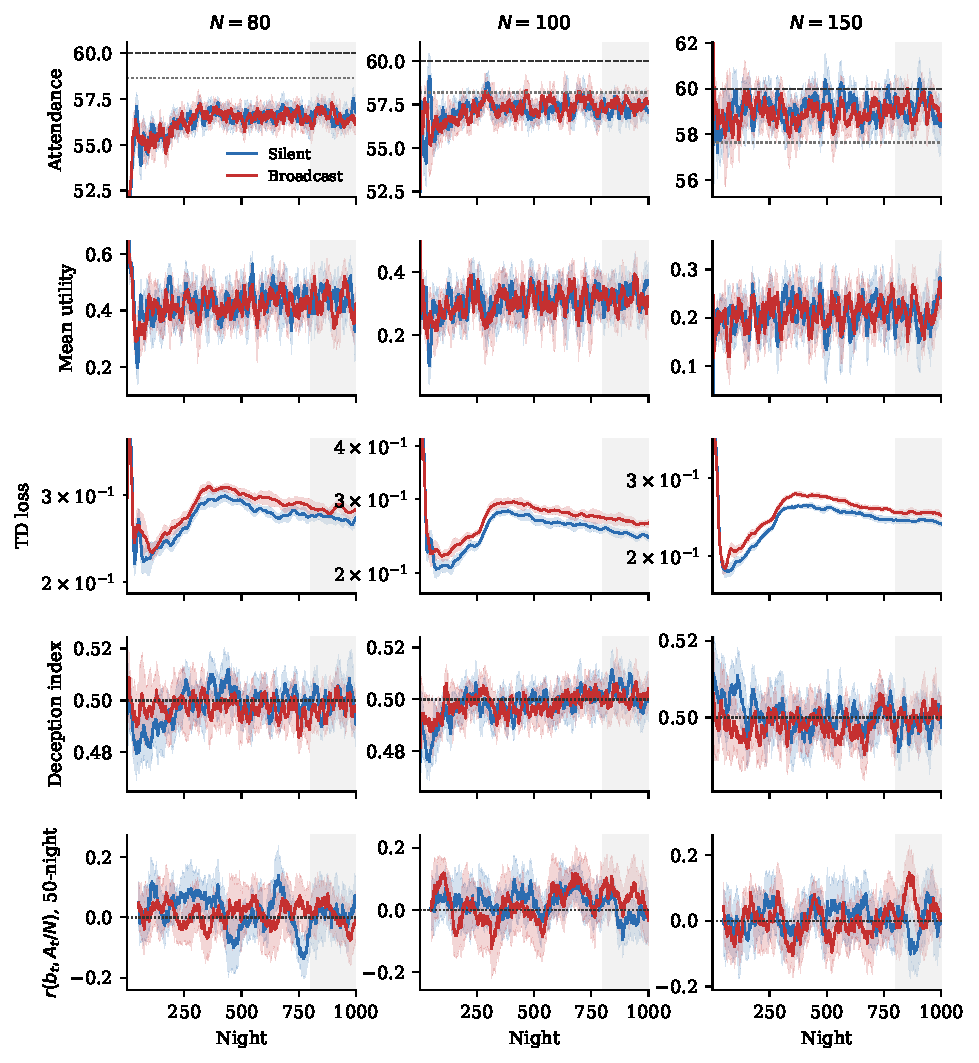
\includegraphics[width=\linewidth]{figures/learning.pdf}
  \caption{Learning over \rnightsLong{} nights: mean across 12 seeds with a 95\% seed-bootstrap band, after a \rsmooth-night moving average (the TD loss is on a log scale). Bottom row: correlation between the share of ``going'' claims and the attendance share over a sliding \rcorrWindow-night window. In the attendance row the dashed line is $A^* = T = 60$ and the dotted line is $Np^*$. The shaded region marks the last \rnightsLate{} nights.}
  \label{fig:learning}
\end{figure}

\subsection{The channel changes nothing, early or late}\label{sec:null}

Table~\ref{tab:contrast} reports the paired contrasts over the last \rnightsLate{} nights. No effect on attendance, utility, distance to equilibrium, regret, efficiency, inequality or strategy entropy is distinguishable from zero after correction. Of the \rnTestsLate{} contrasts, \rnNominalLate{} has $p < 0.05$ and none survives false-discovery-rate control (smallest $q = \rminQLate$). The same holds over all \rnightsLong{} nights (\rnNominalLong{} nominal, none surviving, smallest $q = \rminQLong$) and over the first \rnightsShort{} nights (\rnNominalShort{} nominal, none surviving, smallest $q = \rminQShort$); Appendix~\ref{app:tables} gives both tables. Figure~\ref{fig:contrast} shows the intervals for all three windows. The largest relative change in mean utility in the late window is \rmaxUtilPctLate\%.

\begin{table}[t]
  \centering
  \small
  \setlength{\tabcolsep}{3pt}
  \caption{Silent (S) versus broadcast (B) towns over the last \rnightsLate{} of \rnightsLong{} nights, with the paired difference $\Delta = $ B $-$ S, the exact sign-flip $p$, and the Benjamini--Hochberg $q$ over all \rnTestsLate{} contrasts in this window. Means are over 12 seeds.}
  \label{tab:contrast}
  \resizebox{\linewidth}{!}{%
  \begin{tabular}{l ccccc ccccc ccccc}
    \toprule
    & \multicolumn{5}{c}{$N = 80$} & \multicolumn{5}{c}{$N = 100$} & \multicolumn{5}{c}{$N = 150$} \\
    \cmidrule(lr){2-6}\cmidrule(lr){7-11}\cmidrule(lr){12-16}
    Metric & S & B & $\Delta$ & $p$ & $q$ & S & B & $\Delta$ & $p$ & $q$ & S & B & $\Delta$ & $p$ & $q$ \\
    \midrule
    Mean attendance & 56.64 & 56.51 & $-$0.13 & 0.255 & 0.728 & 57.20 & 57.49 & $+$0.29 & 0.059 & 0.661 & 59.11 & 59.12 & $+$0.01 & 0.927 & 0.948 \\
Deception index & 0.499 & 0.498 & $-$0.001 & 0.803 & 0.948 & 0.503 & 0.501 & $-$0.001 & 0.739 & 0.948 & 0.498 & 0.501 & $+$0.002 & 0.113 & 0.661 \\
Mean utility & 0.437 & 0.435 & $-$0.001 & 0.930 & 0.948 & 0.330 & 0.315 & $-$0.015 & 0.144 & 0.661 & 0.211 & 0.214 & $+$0.003 & 0.462 & 0.866 \\
$|A_t - A^*|$ & 4.84 & 4.91 & $+$0.07 & 0.532 & 0.924 & 5.01 & 4.99 & $-$0.03 & 0.865 & 0.948 & 4.94 & 4.84 & $-$0.10 & 0.396 & 0.866 \\
Mean regret & 0.393 & 0.395 & $+$0.003 & 0.744 & 0.948 & 0.448 & 0.457 & $+$0.009 & 0.188 & 0.661 & 0.469 & 0.465 & $-$0.004 & 0.141 & 0.661 \\
Efficiency & 0.529 & 0.528 & $-$0.001 & 0.930 & 0.948 & 0.458 & 0.437 & $-$0.021 & 0.144 & 0.661 & 0.364 & 0.370 & $+$0.006 & 0.462 & 0.866 \\
Gini (utility) & 0.041 & 0.040 & $-$0.001 & 0.699 & 0.948 & 0.055 & 0.061 & $+$0.006 & 0.056 & 0.661 & 0.093 & 0.095 & $+$0.001 & 0.659 & 0.948 \\
Strategy entropy & 1.846 & 1.849 & $+$0.003 & 0.188 & 0.661 & 1.962 & 1.961 & $-$0.001 & 0.409 & 0.866 & 1.954 & 1.954 & $-$0.000 & 0.900 & 0.948 \\
\bottomrule

  \end{tabular}}
\end{table}

\begin{figure}[t]
  \centering
  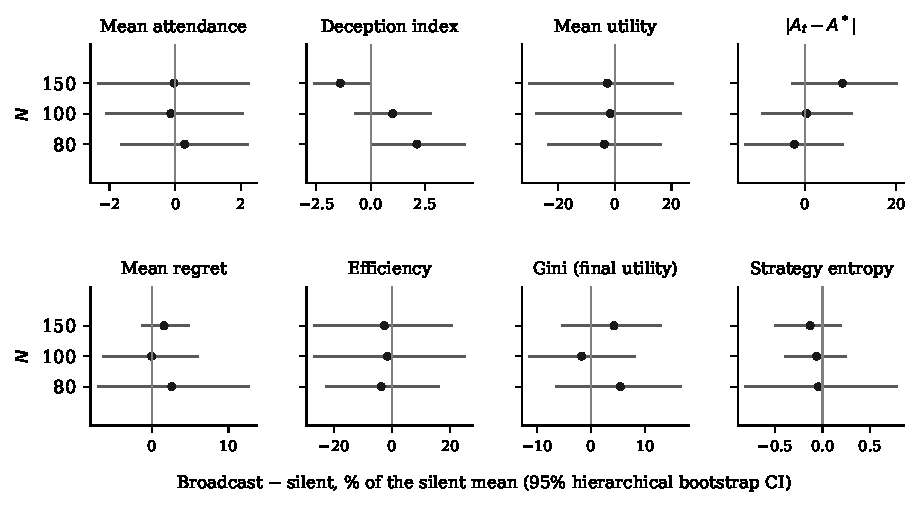
\includegraphics[width=\linewidth]{figures/contrast.pdf}
  \caption{Effect of opening the channel, as a percentage of the silent mean, with 95\% hierarchical bootstrap intervals, for each population size and analysis window.}
  \label{fig:contrast}
\end{figure}

\subsection{The claims carry no information}

Why does a public channel do nothing? Table~\ref{tab:information} answers by looking at the messages. In every condition and at every size, the share of agents claiming ``going'' averages one half, and it is uncorrelated with the share that actually goes. Over the first \rnightsShort{} nights the per-town correlation is \rcorrBcShortLXXX, \rcorrBcShortC{} and \rcorrBcShortCL{} with the channel open, against \rcorrCtlShortLXXX, \rcorrCtlShortC{} and \rcorrCtlShortCL{} when nobody listens. Over the last \rnightsLate{} nights it is \rcorrBcLateLXXX, \rcorrBcLateC{} and \rcorrBcLateCL{}, against \rcorrCtlLateLXXX, \rcorrCtlLateC{} and \rcorrCtlLateCL. None of the paired differences is significant (late window: $p = \rcorrPLateLXXX$, $\rcorrPLateC$ and $\rcorrPLateCL$). Broadcast towns lean slightly positive late in training, but the effect is small, inconsistent across seeds and not distinguishable from zero. An agent that conditioned on $b_t$ would learn almost nothing from it, and the right panel of Figure~\ref{fig:minds} shows the resulting cloud.

\begin{table}[t]
  \centering
  \small
  \setlength{\tabcolsep}{4pt}
  \caption{The content of the claims. $r(b_t, A_t/N)$ is the per-town correlation between the share of ``going'' claims and the attendance share (mean $\pm$ s.d.\ over 12 seeds), over the first \rnightsShort{} nights and over the last \rnightsLate{} of \rnightsLong. The remaining columns refer to the last \rnightsLate{} nights: the mean claim share, the per-agent-night rates of each kind of lie, and the standard deviation of attendance.}
  \label{tab:information}
  \begin{tabular}{rlcccccc}
    \toprule
    & & \multicolumn{2}{c}{$r(b_t, A_t/N)$} & \multicolumn{4}{c}{Last \rnightsLate{} nights} \\
    \cmidrule(lr){3-4}\cmidrule(lr){5-8}
    $N$ & Condition & First \rnightsShort & Last \rnightsLate & Mean $b_t$ & Bluff & Covert & SD$(A_t)$ \\
    \midrule
    80 & Silent & $+$0.045 $\pm$ 0.124 & 0.500 & 0.150 & 0.336 & 7.39 \\
80 & Broadcast & $+$0.020 $\pm$ 0.117 & 0.492 & 0.151 & 0.346 & 6.77 \\
100 & Silent & $+$0.025 $\pm$ 0.083 & 0.499 & 0.211 & 0.276 & 7.80 \\
100 & Broadcast & $+$0.059 $\pm$ 0.103 & 0.496 & 0.212 & 0.279 & 8.58 \\
150 & Silent & $-$0.003 $\pm$ 0.127 & 0.500 & 0.307 & 0.199 & 7.41 \\
150 & Broadcast & $-$0.002 $\pm$ 0.078 & 0.494 & 0.301 & 0.198 & 8.55 \\
\bottomrule

  \end{tabular}
\end{table}

\subsection{Independence explains the deception index}

If a claim is independent of the action and says ``going'' with probability $q$, the probability of a lie is
\begin{equation}
\Pr[\text{lie}] = q\,(1 - \pi) + (1 - q)\,\pi,
\end{equation}
where $\pi$ is the probability of going. At $q = \tfrac12$ this is exactly $\tfrac12$ for any $\pi$. That is what we observe. Over the last \rnightsLate{} nights the deception index is \rdecCtlLateLXXX, \rdecCtlLateC{} and \rdecCtlLateCL{} in silent towns, where nobody could be deceived, and \rdecBcLateLXXX, \rdecBcLateC{} and \rdecBcLateCL{} in broadcast towns. Over the first \rnightsShort{} nights it is \rdecCtlShortLXXX, \rdecCtlShortC{} and \rdecCtlShortCL{} against \rdecBcShortLXXX, \rdecBcShortC{} and \rdecBcShortCL.

The same independence predicts the \emph{kind} of lie. Bluffs occur at rate $q(1-\pi)$ and covert visits at rate $(1-q)\pi$, so their mix depends only on attendance. In small towns most agents go, so covert visits dominate: \rcovertBcLateLXXX{} versus \rbluffBcLateLXXX{} at $N = 80$ in the last \rnightsLate{} nights. In large towns most stay home, so bluffs dominate: \rbluffBcLateCL{} versus \rcovertBcLateCL{} at $N = 150$. The silent towns show the same pattern (Table~\ref{tab:information}). A naive reading of the broadcast data would call large towns ``bluffers'' and small towns ``sneaks''; in fact both are the arithmetic of uninformative claims.

\subsection{Who lies is set by temperament at first, and then by nothing}

Early in training, an agent's lie rate is strongly and negatively rank-correlated with its honesty trait (Figure~\ref{fig:minds}, left). Over the first \rnightsShort{} nights the Spearman $\rho$ is \rrhoBcShortLXXX, \rrhoBcShortC{} and \rrhoBcShortCL{} in broadcast towns, and \rrhoCtlShortLXXX, \rrhoCtlShortC{} and \rrhoCtlShortCL{} in silent towns. The correlation is just as strong where lying cannot benefit anyone, so it reflects the claim--action coupling each agent is initialised with, not a strategic choice. Training removes it. Over the last \rnightsLate{} nights $\rho$ is \rrhoBcLateLXXX, \rrhoBcLateC{} and \rrhoBcLateCL{} in broadcast towns and \rrhoCtlLateLXXX, \rrhoCtlLateC{} and \rrhoCtlLateCL{} in silent towns (Figure~\ref{fig:minds}, centre): every agent ends up lying about half the time, whatever its temperament. Honest agents still end with a slightly better public reputation in broadcast towns (a gap of \rrepgapBcLateLXXX, \rrepgapBcLateC{} and \rrepgapBcLateCL{} over the last \rnightsLate{} nights). Reputation here is computed directly from truthfulness, so the gap records who told the truth rather than any effect of reputation on behaviour.

\begin{figure}[t]
  \centering
  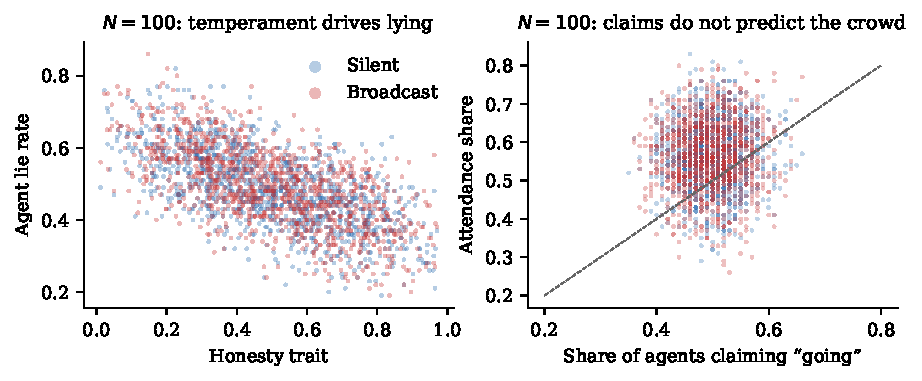
\includegraphics[width=\linewidth]{figures/minds.pdf}
  \caption{$N = 100$, all 12 seeds. Left and centre: each agent's honesty trait against its lie rate over the first \rnightsShort{} nights and over the last \rnightsLate{} of \rnightsLong. Right: the share of ``going'' claims against the share that went over the last \rnightsLate{} nights, one point per night.}
  \label{fig:minds}
\end{figure}

\section{Discussion}

\paragraph{Babbling as the learned outcome.}
In El Farol, a credible ``going'' claim would push others to stay home, which is good for the speaker. That makes the claim not credible: every agent wants to say ``going'' whatever it does. Under such conflicting interests, cheap-talk theory predicts that informative messaging unravels and babbling remains \citep{crawford1982,farrell1996}. Our independent learners arrive at the same place without anyone imposing it, and stay there: the claims carry no information after \rnightsShort{} nights and none after \rnightsLong. The speaker network gets no reward for informativeness, and the listeners have nothing to learn from noise. This matches the negotiation result of \citet{cao2018}, here at population scale and with zero shared parameters. The long run also separates two readings of the short one. Agents that had simply not yet learned to use the channel would start to use it as training continues; ours do not.

\paragraph{Coordination does not need talk.}
Even without a channel, attendance stays within a few seats of the comfort line, and learning brings it closer: averaged over both conditions at $N = 100$, $|A_t - A^*|$ falls from \rgapEarlyC{} seats in the first \rnightsShort{} nights to \rgapLateC{} in the last \rnightsLate. Each agent's private history of attendance and payoffs carries the information that coordination needs. A public channel that adds nothing on top of it cannot help.

\paragraph{Measuring deception in learning systems.}
A deception index near $0.5$ in a talking population is easy to read as rampant, strategic lying. Our silent control shows the same number with no audience at all. Any study of learned deception needs a condition in which nobody can be deceived, and should test whether claims predict behaviour before interpreting the rate of mismatches.

\paragraph{Limitations.}
Claims are binary and the only published statistic is their mean, so agents cannot build reputations for specific individuals. The actors learn from counterfactual payoffs, which is a strong form of feedback. The TD loss does not converge, which is expected when every agent's targets move with the others' policies; our convergence statements refer to behaviour, not to the loss. We ran \rnightsLong{} nights; even longer horizons, richer messages, identity-tagged broadcasts or shared rewards could still produce informative talk. Our sign-flip tests have a resolution of $2/4096$ with 12 seeds, and the treatment effects we rule out are small but not zero. We test three overlapping windows of the same runs, so they are not independent replications.

\section{Reproducibility and the interactive reference}\label{sec:repro}

Every number, table and figure in the results is generated from the raw output of the runs by \texttt{paper/analysis.py}. The sweep is run by \texttt{paper/run\_sweep.sh}, which calls \texttt{experiment.py} for every town and then \texttt{analyzer.py} for the full-run and late-window statistics of each population size. The reference engine is written in PyTorch and runs on CPU or GPU.

We also ported the learning engine to TypeScript so that it runs entirely in a web browser, on a laptop or a phone, alongside an interactive three-dimensional view of the town. The port keeps the network architecture, initialisation, policy, replay, losses, target networks, gradient clipping and optimiser of the reference. The browser runs the original \texttt{analyzer.py} through Pyodide \citep{pyodide}. In a separate check on paired seeds, the port and the PyTorch engine did not differ significantly on mean attendance, deception, utility, rerouting or final TD loss. Their random streams differ, so individual seeds are not bit-identical, and none of the results in this paper come from the port. Code and the live reference are available at \url{https://github.com/FABASTIC/ElFarolProblem} and \url{https://el-farol-rho.vercel.app}.

\section{Conclusion}

Give a population of independent deep Q-learners a public channel in the El Farol problem and they learn to ignore it. Their claims settle at a coin flip that is independent of what they do, so the channel changes neither coordination nor welfare. The apparent deception rate of one half is the arithmetic of uninformative talk, not strategy. Cheap talk at El Farol stays cheap.

\bibliographystyle{plainnat}
\bibliography{refs}

\appendix

\section{Contrast tables for the other windows}\label{app:tables}

\begin{table}[h]
  \centering
  \small
  \setlength{\tabcolsep}{3pt}
  \caption{As Table~\ref{tab:contrast}, over all \rnightsLong{} nights. $q$ is computed over the \rnTestsLong{} contrasts in this window.}
  \label{tab:contrast-long}
  \resizebox{\linewidth}{!}{%
  \begin{tabular}{l ccccc ccccc ccccc}
    \toprule
    & \multicolumn{5}{c}{$N = 80$} & \multicolumn{5}{c}{$N = 100$} & \multicolumn{5}{c}{$N = 150$} \\
    \cmidrule(lr){2-6}\cmidrule(lr){7-11}\cmidrule(lr){12-16}
    Metric & S & B & $\Delta$ & $p$ & $q$ & S & B & $\Delta$ & $p$ & $q$ & S & B & $\Delta$ & $p$ & $q$ \\
    \midrule
    Mean attendance & 56.31 & 56.27 & $-$0.04 & 0.382 & 0.615 & 57.19 & 57.25 & $+$0.06 & 0.245 & 0.542 & 59.11 & 58.96 & $-$0.15 & 0.035 & 0.375 \\
Deception index & 0.498 & 0.497 & $-$0.001 & 0.782 & 0.844 & 0.498 & 0.498 & $+$0.000 & 0.828 & 0.854 & 0.500 & 0.499 & $-$0.002 & 0.177 & 0.542 \\
Mean utility & 0.427 & 0.420 & $-$0.007 & 0.030 & 0.375 & 0.310 & 0.304 & $-$0.006 & 0.062 & 0.375 & 0.208 & 0.210 & $+$0.002 & 0.342 & 0.611 \\
$|A_t - A^*|$ & 5.24 & 5.28 & $+$0.03 & 0.557 & 0.694 & 5.46 & 5.51 & $+$0.04 & 0.549 & 0.694 & 5.21 & 5.32 & $+$0.11 & 0.090 & 0.424 \\
Mean regret & 0.400 & 0.404 & $+$0.005 & 0.051 & 0.375 & 0.461 & 0.464 & $+$0.003 & 0.214 & 0.542 & 0.471 & 0.470 & $-$0.000 & 0.822 & 0.854 \\
Efficiency & 0.518 & 0.509 & $-$0.009 & 0.030 & 0.375 & 0.430 & 0.422 & $-$0.008 & 0.062 & 0.375 & 0.359 & 0.362 & $+$0.003 & 0.342 & 0.611 \\
Gini (utility) & 0.022 & 0.022 & $-$0.000 & 0.923 & 0.923 & 0.028 & 0.027 & $-$0.001 & 0.261 & 0.542 & 0.044 & 0.043 & $-$0.001 & 0.540 & 0.694 \\
Strategy entropy & 1.848 & 1.849 & $+$0.001 & 0.263 & 0.542 & 1.960 & 1.960 & $-$0.001 & 0.314 & 0.610 & 1.953 & 1.952 & $-$0.001 & 0.030 & 0.375 \\
\bottomrule

  \end{tabular}}
\end{table}

\begin{table}[h]
  \centering
  \small
  \setlength{\tabcolsep}{3pt}
  \caption{As Table~\ref{tab:contrast}, over the first \rnightsShort{} nights. $q$ is computed over the \rnTestsShort{} contrasts in this window.}
  \label{tab:contrast-short}
  \resizebox{\linewidth}{!}{%
  \begin{tabular}{l ccccc ccccc ccccc}
    \toprule
    & \multicolumn{5}{c}{$N = 80$} & \multicolumn{5}{c}{$N = 100$} & \multicolumn{5}{c}{$N = 150$} \\
    \cmidrule(lr){2-6}\cmidrule(lr){7-11}\cmidrule(lr){12-16}
    Metric & S & B & $\Delta$ & $p$ & $q$ & S & B & $\Delta$ & $p$ & $q$ & S & B & $\Delta$ & $p$ & $q$ \\
    \midrule
    Mean attendance & 54.84 & 55.00 & $+$0.16 & 0.521 & 0.775 & 56.40 & 56.33 & $-$0.08 & 0.723 & 0.826 & 58.71 & 58.68 & $-$0.02 & 0.958 & 0.958 \\
Deception index & 0.486 & 0.496 & $+$0.010 & 0.041 & 0.287 & 0.487 & 0.492 & $+$0.005 & 0.181 & 0.569 & 0.506 & 0.499 & $-$0.007 & 0.015 & 0.287 \\
Mean utility & 0.402 & 0.387 & $-$0.015 & 0.230 & 0.608 & 0.261 & 0.257 & $-$0.004 & 0.488 & 0.775 & 0.192 & 0.187 & $-$0.005 & 0.330 & 0.748 \\
$|A_t - A^*|$ & 7.18 & 7.02 & $-$0.17 & 0.477 & 0.775 & 7.61 & 7.63 & $+$0.03 & 0.882 & 0.924 & 6.79 & 7.35 & $+$0.56 & 0.043 & 0.287 \\
Mean regret & 0.424 & 0.434 & $+$0.011 & 0.179 & 0.569 & 0.502 & 0.502 & $-$0.000 & 0.956 & 0.958 & 0.485 & 0.493 & $+$0.008 & 0.054 & 0.322 \\
Efficiency & 0.487 & 0.469 & $-$0.018 & 0.230 & 0.608 & 0.362 & 0.357 & $-$0.006 & 0.488 & 0.775 & 0.331 & 0.322 & $-$0.009 & 0.330 & 0.748 \\
Gini (utility) & 0.059 & 0.062 & $+$0.003 & 0.160 & 0.569 & 0.106 & 0.104 & $-$0.002 & 0.539 & 0.775 & 0.154 & 0.161 & $+$0.007 & 0.181 & 0.569 \\
Strategy entropy & 1.856 & 1.855 & $-$0.001 & 0.824 & 0.891 & 1.953 & 1.951 & $-$0.001 & 0.516 & 0.775 & 1.948 & 1.945 & $-$0.003 & 0.198 & 0.595 \\
\bottomrule

  \end{tabular}}
\end{table}

\end{document}
